% -*- coding: utf-8 -*-
% !TEX root = ../main.tex

% TODO Présentation des travaux précédents pour expliquer d'où on part (programmes existants, études...)
% TODO Présenter les outils utilisés (logiciel/application, supercalculateur, langage de programmation...)
% Les sous-parties suivantes servent d'exemple, vous n'êtes pas obligés de les reprendre

\subsection{Concept du format de trace PALLAS}\label{ssec:pallas_status}

Les formats de trace classiques tels que \verb!OTF2! optimisent l'enregistrement et le compression de la trace mais ne permettent pas une factorisation réalisée lors de l'exécution du programme 
et ne ne permettent pas une macro-analyse efficace de la trace. En effet, \verb!OTF2! stocke les données d'exécution de manière linéaire, ce qui rend l'analyse de la trace très fastidieuse.\newline
Ainsi, \verb!PALLAS! sépare la trace en deux parties : l'une permettant une analyse structurelle de la trace et l'autre permettant un stockage précis des différents évènements.
Le poids total sur le disque est causé majoritairement par le stockage précis des évènements, donc le fait de stocker certaines informations plus "légères" séparément permet de ne pas 
avoir à charger la trace systématiquement pout toutes les analyses de cette dernière.\newline
Les évènements sont enregistrés par threads et stockés sous formes de tokens de manière hièrarchique : évènements, boucles et séquences.\newline
La détection des boucles est quant à elle en complexité $O(n^2)$ qui peut être bornée avec une longueur maximale, voire désactivée pour des applications trop irrégulières.

\subsubsection{Stockage hiérarchique des données}\label{ssec:hierarchy}

Il y a d'un côté les fichiers contenant tous les détails de l'exécution comme les durées et les timestamps de chaque évènement, regroupés par token. \newline
De l'autre côté il y a un fichier beaucoup plus léger de structure qui permet d'avoir un résumé de la grammaire des tokens (évènements, séquences, boucles) ainsi que des statistiques
sur les différents données (durées minimales, maximales et moyennes). Ce fichier de structure permet de réaliser une macro-analyse post-mortem rapide et efficace de la trace sans devoir charger celle-ci en entier.\newline
Le stockage des données lors de l'exécution du programme se fait grâce à une structure de vecteurs, décomposés en sous-vecteurs de taille fixe. 
Ces vecteurs sont de deux types différents : d'un côté il y a les vecteurs permettant de stocker les différentes séquences qui peuvent être plus ou moins longues; de l'autre côté
il y a les vecteurs de timestamps (indicateurs de temporalité) qui sont en grande partie responsables du poids de la trace et sont donc compressés.\\
Actuellement, l'écriture et la compression des données se fait en fin d'exécution. La compression par défaut est celle de l'algorithme \verb!ZSTD! qui est sans perte, mais d'autres sont 
proposés comme \verb!ZFP! qui sont avec perte. Un flush régulier pendant l'exécution serait également possible.

\subsubsection{Outils d'analyse fournis avec PALLAS}\label{ssec:analysis_tools}

Enfin, \verb!PALLAS! fournit des outils d'analyse de la trace déjà implémentés tels que: 
\begin{itemize}
    \item \verb!pallas_print! qui permet d'explorer toute la trace en l'affichant.
    \item \verb!pallas_contention! qui calcule le score de contention (indicateur permettant de quantifier le nombre de threads se partageant la même ressource) en utilisant uniquement les fichiers de structure (donc sans charger toute la trace).
    \item \verb!pallas_comm_matrix! qui réalise une matrice de communication (identifiant quels processus s'échangent des données) MPI (Message Passing Interface) en n'utilisant également que la structure de la trace.
    \item \verb!pallas_histogram! qui extrait la distribution des durées grace à un accès précis aux vecteurs de durées concernés.
\end{itemize}

Le premier article \cite{pallas_ipdps} publié présentant \verb!PALLAS! montre que ces outils sont biens plus efficaces avec le format de trace \verb!PALLAS! qu'avec d'autres formats existants.

Voici un exemple~\ref{fig:comm} de résultats liés au calcul d'une matrice de communications \verb!MPI!~\cite{pallas_ipdps}, où l'on constate l'intérêt d'utiliser \verb!PALLAS! pour des traces à large échelle :

\begin{figure}[!h]
    \centering
    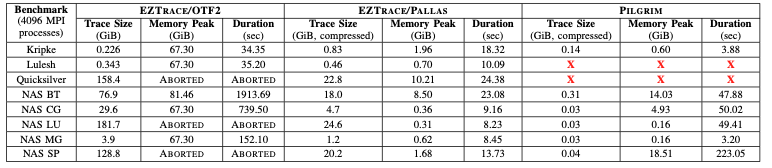
\includegraphics[width=1\textwidth]{img/comm.png}
    \caption{Statistiques sur le calcul de matrice de communications MPI avec plusieurs formats de trace}
    \label{fig:comm}
\end{figure}

\subsection{Outils utilisés}\label{ssec:outils}

Les travaux réalisés lors de ce stage ont été mis en place sur la machine \verb!Sandor! de \gls{tsp}.
\verb!Sandor! est un serveur de calcul équipé de deux processeurs physiques, 
offrant au total 64 c\oe{}urs et 128 threads.
Elle dispose de 504 \gls{go} de mémoire vive, ce qui en fait une plateforme adaptée aux charges de calcul intensives.\par
De plus, les applications \verb!MPI! utilisés comme benchmarks sont : LULESH et NAS BT, LU, MG, FT, CG, SP lancées sur 64 c\oe{}urs.

Les deux configuration utilisées sont : 
\begin{itemize}
    \item Vanilla : on exécute l'application sans outil de traçage
    \item \verb!EZTrace!/\verb!PALLAS! : on trace à l'aide de l'outil \verb!EZTrace! en utilisant le format de trace \verb!PALLAS!
\end{itemize}

Afin d'étudier la compression, on utilisera également le programme \verb!pallas_editor! qui permet de passer d'une trace compressée avec un algorithme A à une trace compressée avec
un algorithme B.
